\section{作业题目：结构力学基础与技巧班第1次作业（几何组成分析）}
\begin{analysisbox}
先算自由度，再按二元体、两刚片、三刚片和瞬变判据复核。判断顺序建议为：先找可并入大地的刚片，再检查约束方向是否共线、平行或交于一点，最后判定有无多余约束。
\end{analysisbox}
\subsection*{第 1 页转写}
几何组成分析作业及答案

1-1图1-56所示体系的几何组成为（

）。（浙江大学2008）

A：几何瞬变，无多余约束

B.几何不变

C.几何常变

D.几何瞬变，有多余约束

1-2欲使图1-57所示体系成为无多余约束的几何不变体系，则需在A端加人（，

（中南大学2011，合肥工业大学2009）

A.固定铰支座

B.固定支座

C.滑动铰支座

D.定向支座

1-3图1-58所示体系的几何构造性质是（

）。（中南大学2009）

A.常变体系

B.瞬变体系

C.无多余联系的几何不变体系

D.有多余联系的几何不变体系

图1-56

图1-57

图1-58

1-4

图1-59所示体系内部是

体系，它有

个多余约束。（广西大学

2010)

1-5

图1-60所示体系的计算自由度W=

（哈尔滨工业大学2011）

1-6

图1-61所示体系几何不变且有多余联系。（

）（中南大学2012)
\begin{figure}[H]\centering
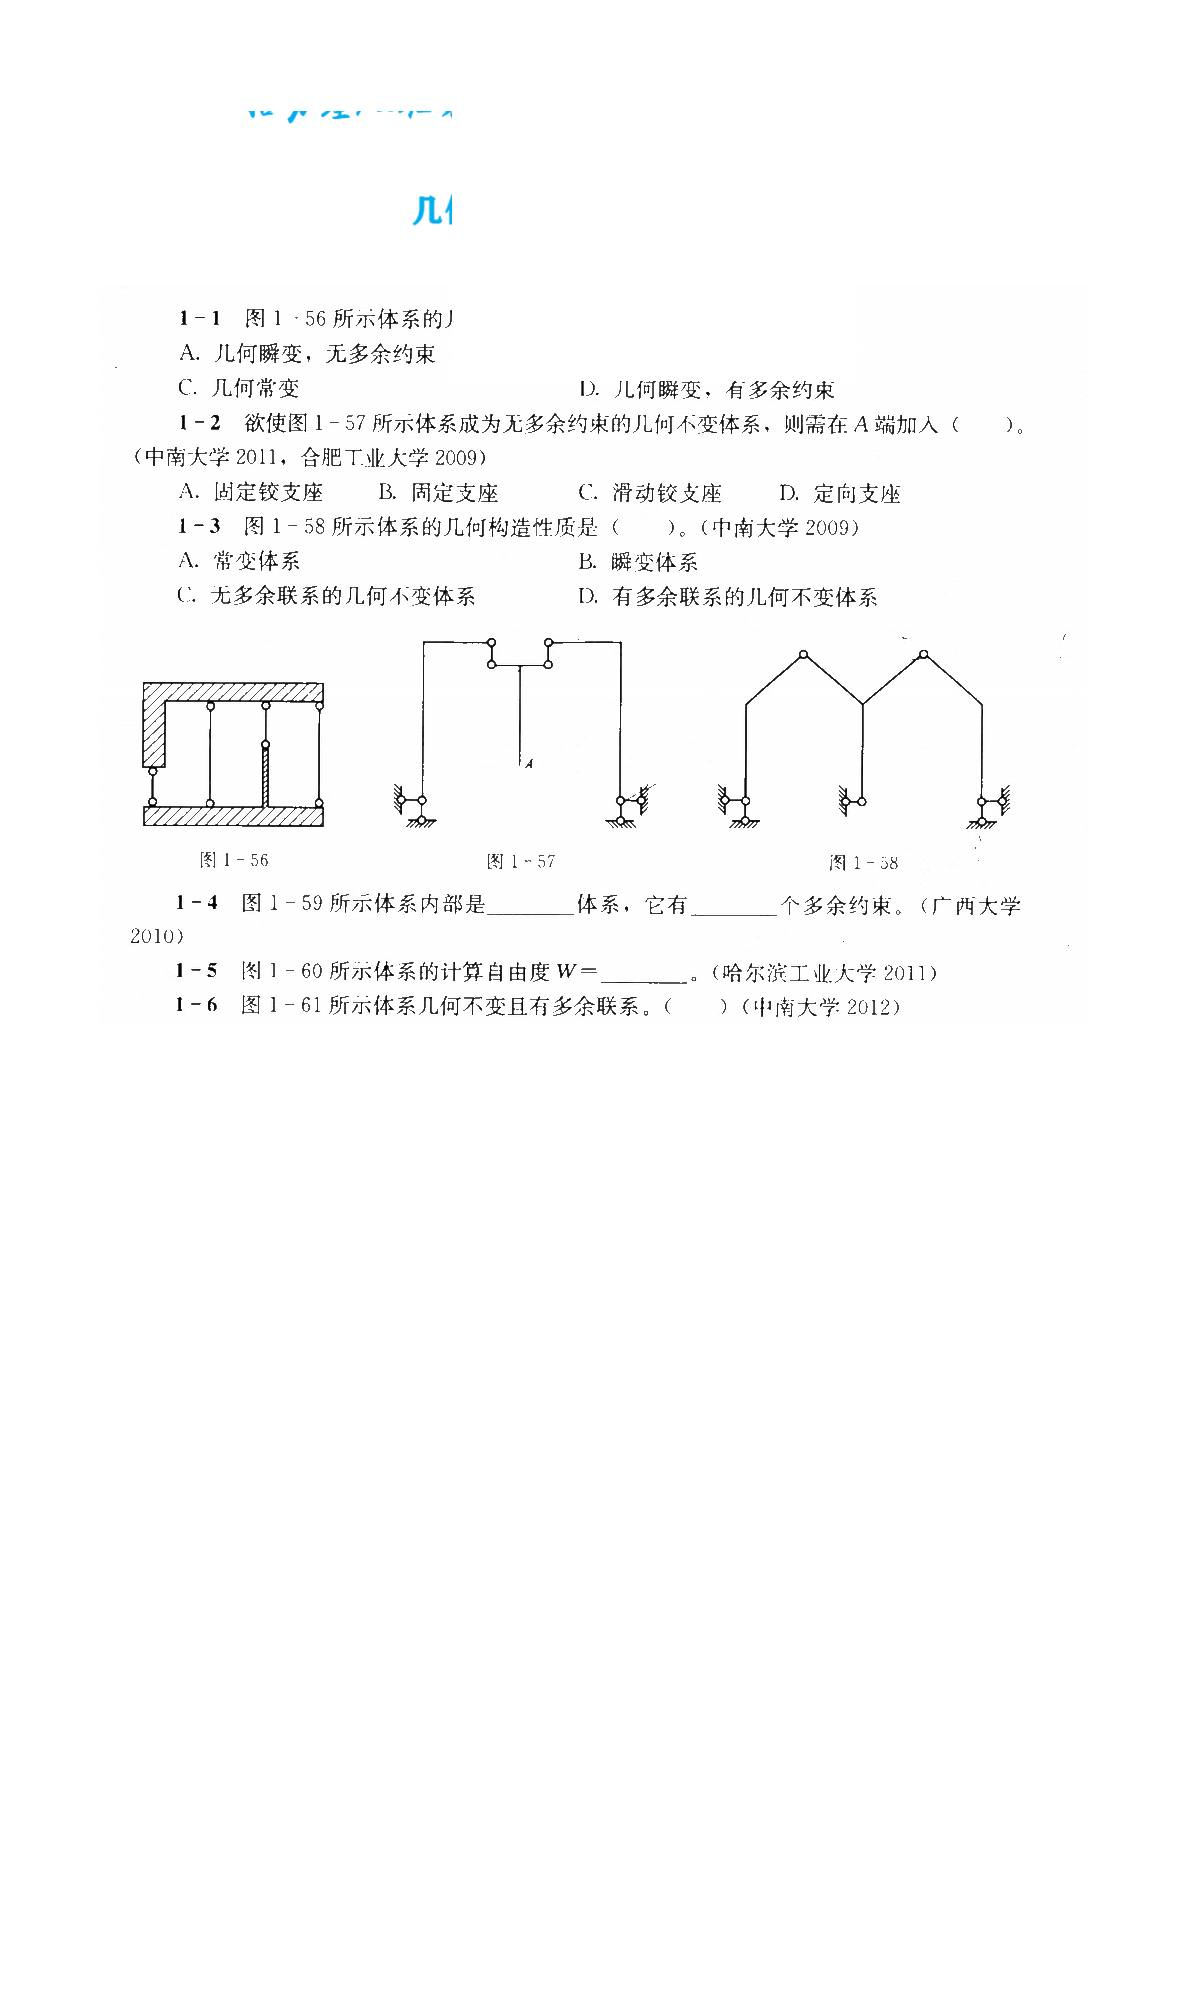
\includegraphics[width=0.92\textwidth]{figures/src02_p001.jpg}
\caption{结构力学基础与技巧班第1次作业（几何组成分析） 第 1 页清理图形页}
\end{figure}
\subsection*{第 2 页转写}
图1-60

图1-59

图1-61

1-7

对图1-62所示体系进行几何组成分析。（哈尔滨工业大学2009）

1-8

对图1-63所示体系作几何组成分析。（武汉科技大学2009）

1-9

对图1-64所示杆件体系进行几何构造分析。（武汉理工大学2008）

图1-63

图1-62

图1-64

1-10

计算图1-65所示体系的计算自由度，试分析其体系的几何组成。（华南理工大

学2012)

1-11

对图1-66所示平面体系进行几何组成分析，并指出结构超静定次数。（青岛理

工大学2012)

图1-65

图1-66

1- 12

分析图1－67所示体系的几何稳定性，写出分析过程。（东南大学2008）

1 - 13

试对图1-68所示体系作几何组成分析。（山东建筑大学2011）

图1-67

图1-68
\begin{figure}[H]\centering
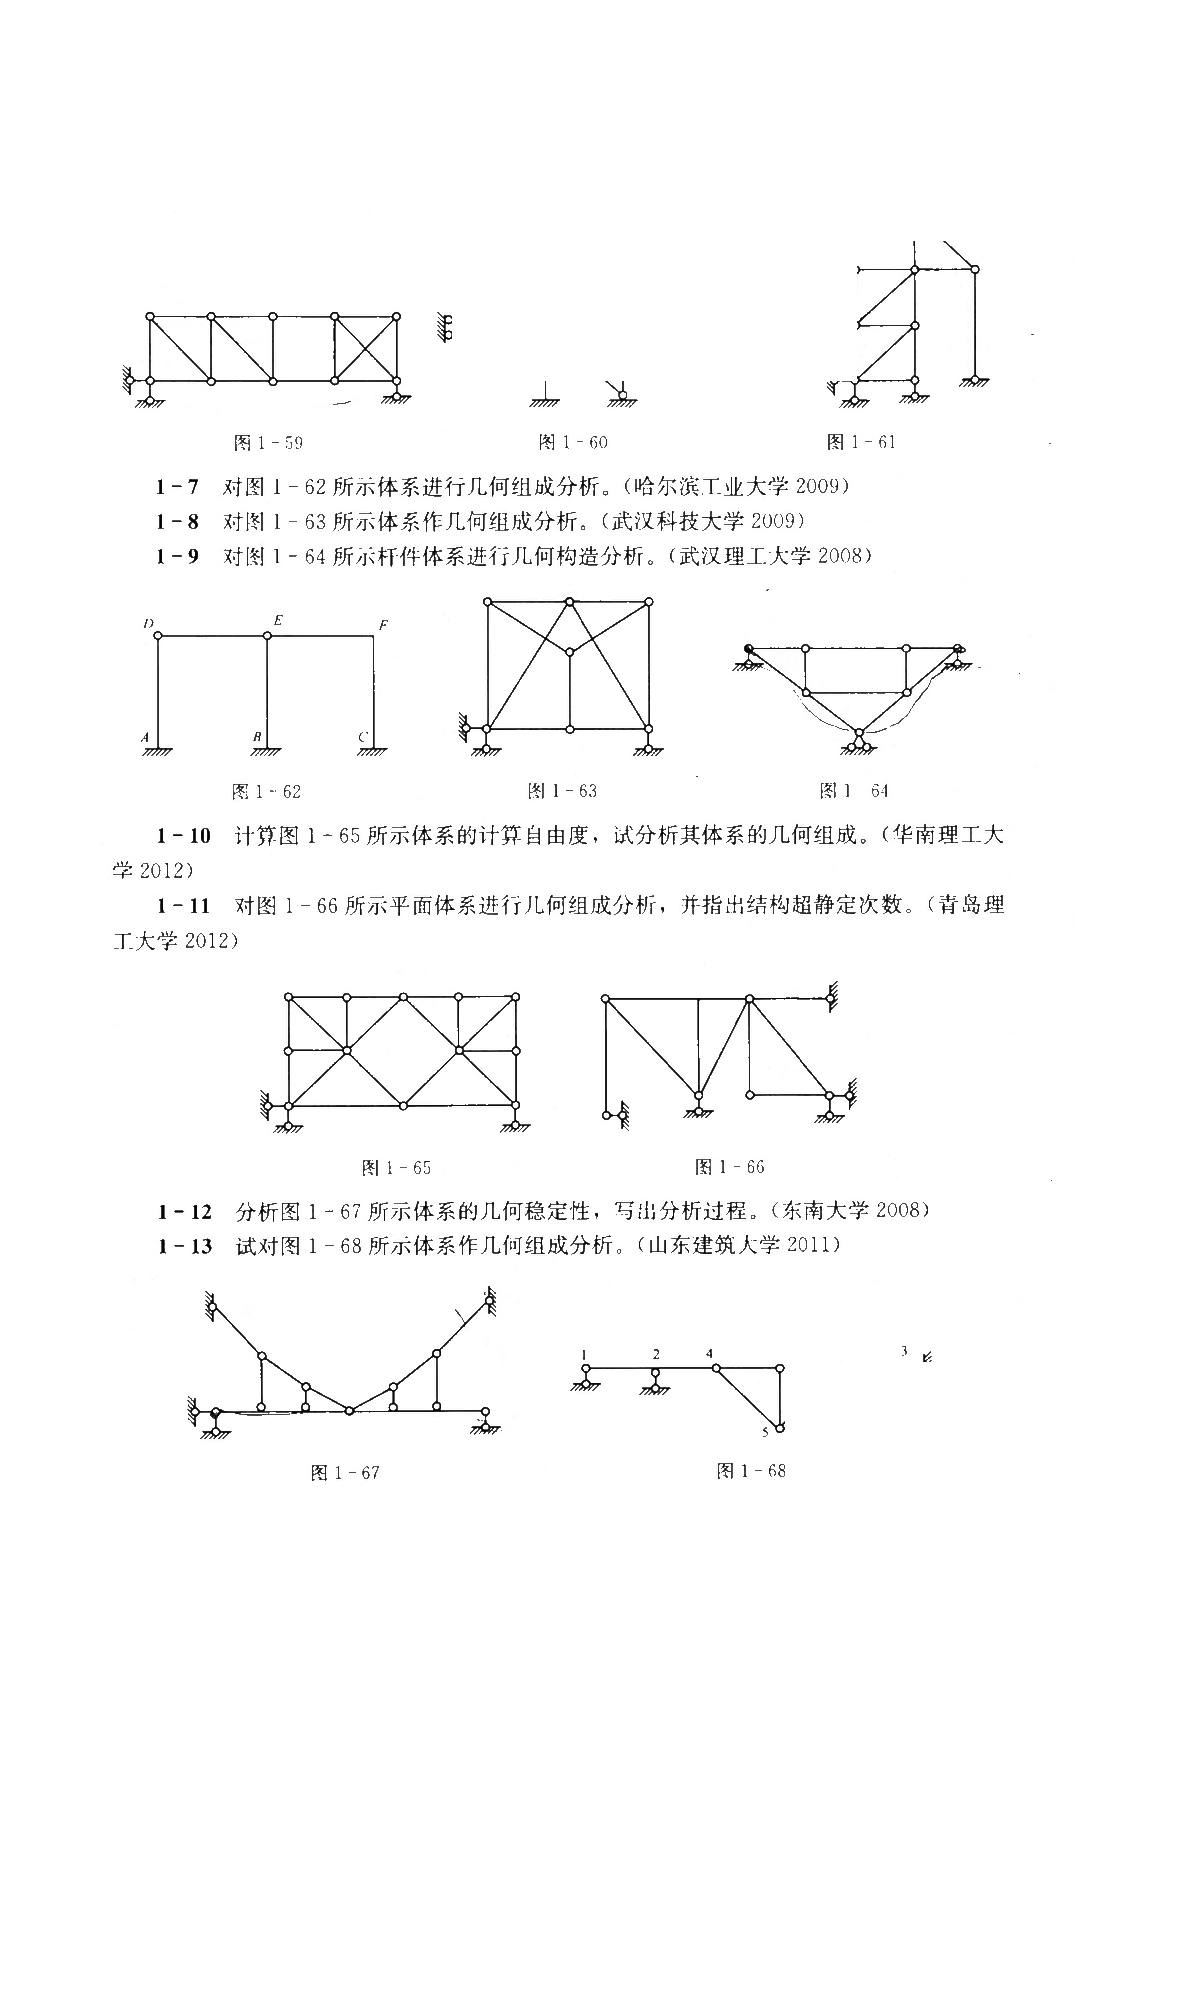
\includegraphics[width=0.92\textwidth]{figures/src02_p002.jpg}
\caption{结构力学基础与技巧班第1次作业（几何组成分析） 第 2 页清理图形页}
\end{figure}
\subsection*{第 3 页转写}
1-14

试对图1－69所示体系作几何组成分析。（山东建筑大学2008）

1- 15

计算图1-70的计算自由度，并作几何构造分析。（中国地震局工程力学研究所

2010)

图1-69

图1-70

1-16

对图1－71所示体系进行几何构造分析。（西南交通大学2008）

1-17

计算图1-72所示体系的计算自由度，并进行几何构成分析。（北京工业大学

2010)

图1-71

图1-72
\begin{figure}[H]\centering
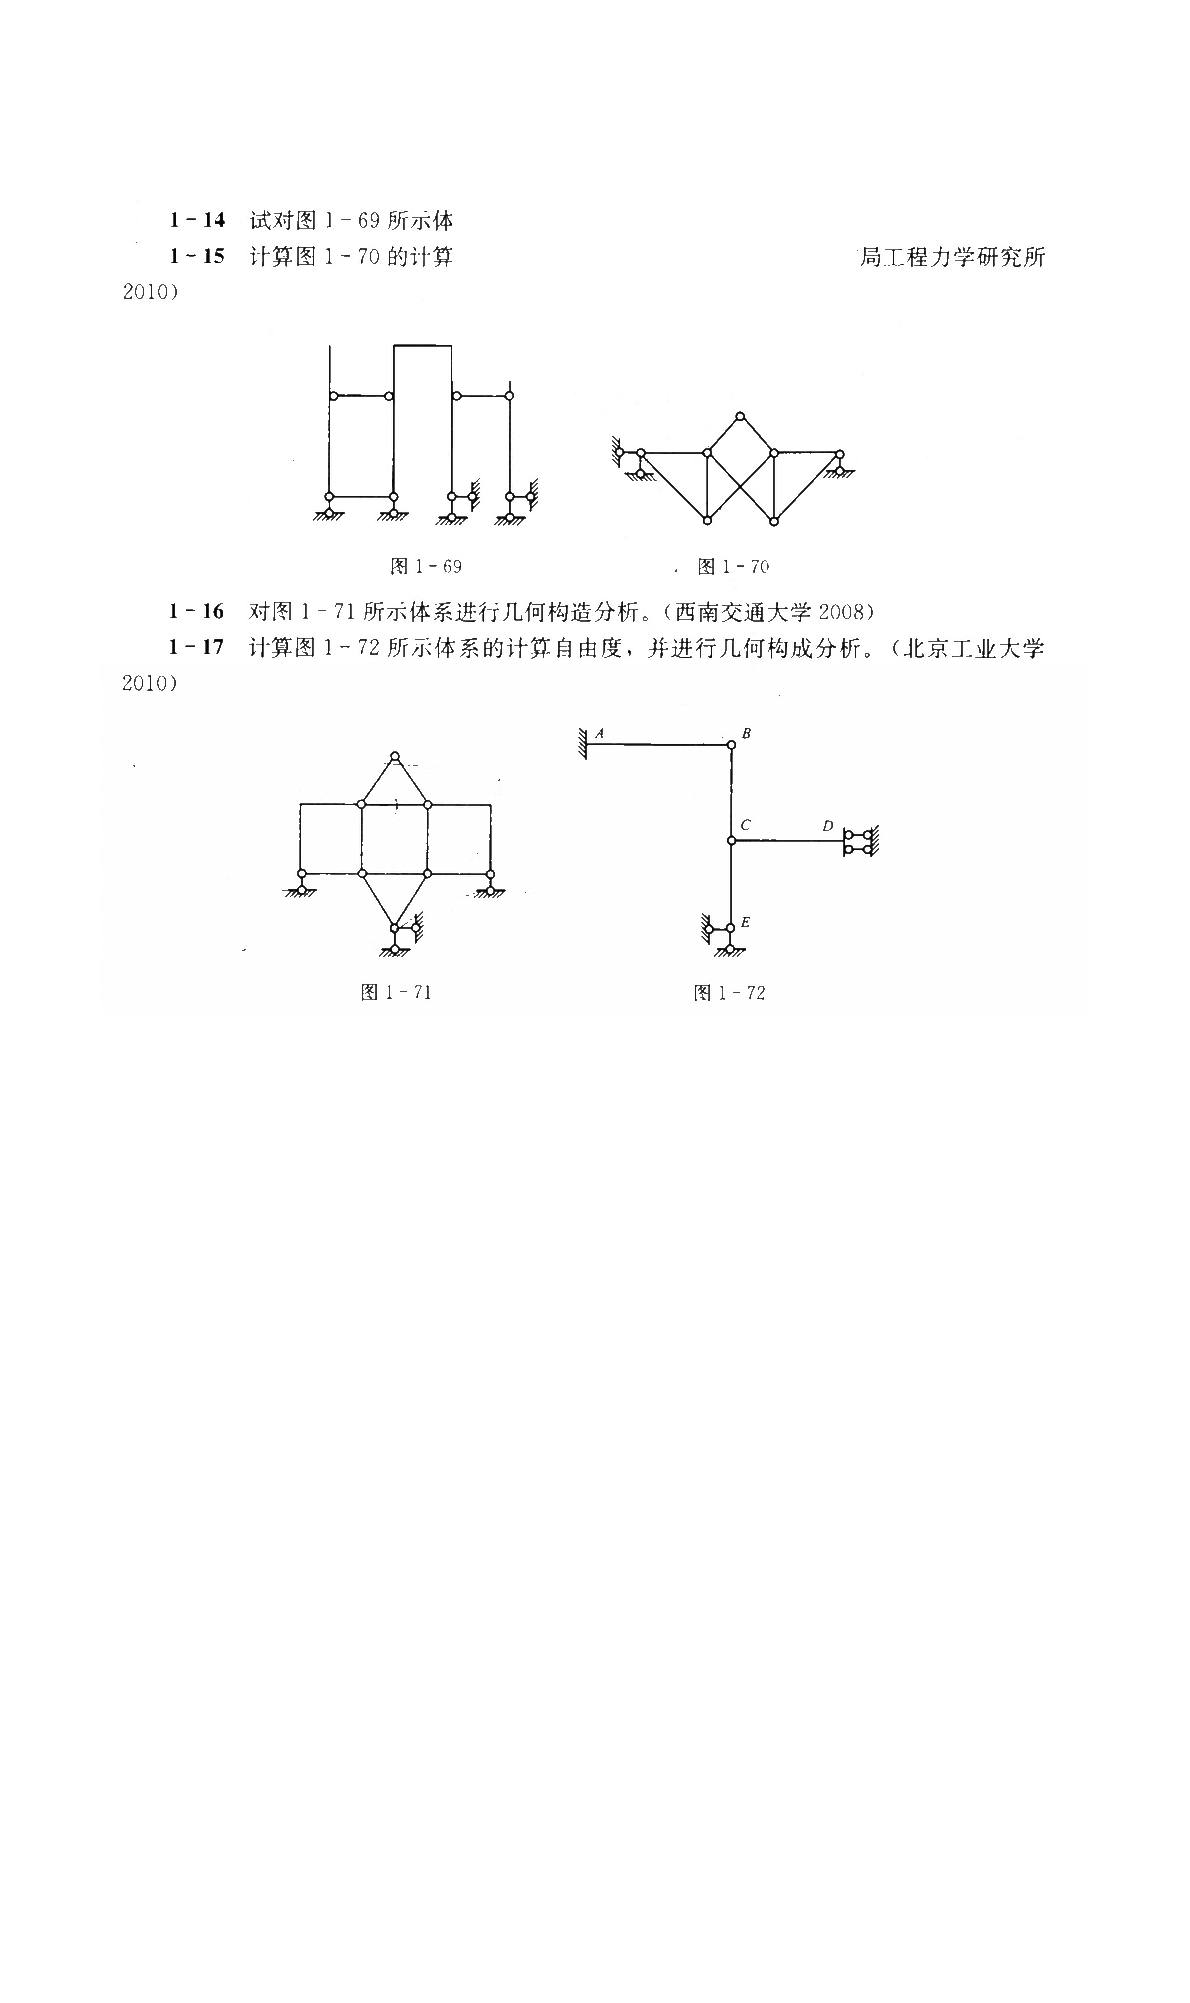
\includegraphics[width=0.92\textwidth]{figures/src02_p003.jpg}
\caption{结构力学基础与技巧班第1次作业（几何组成分析） 第 3 页清理图形页}
\end{figure}
